\documentclass[11pt]{article}

\usepackage[margin=1in]{geometry}
\usepackage{graphicx}
\usepackage{booktabs}
\usepackage{amsmath}
\usepackage{xcolor}
\usepackage{listings}
\usepackage{float}
\usepackage[hidelinks]{hyperref}
\usepackage{caption}
\captionsetup{font=small,labelfont=bf}

\definecolor{codebg}{gray}{0.96}
\lstdefinestyle{chat}{
  basicstyle=\ttfamily\footnotesize,
  backgroundcolor=\color{codebg},
  frame=single, rulecolor=\color{gray!40},
  breaklines=true, columns=fullflexible,
  showstringspaces=false, xleftmargin=4pt, xrightmargin=4pt,
  literate={<}{{\textless}}1 {>}{{\textgreater}}1 {|}{{\textbar}}1
}

\title{\textbf{Tracing Eval-Awareness Emergence Through OLMo-3 Training}\\[2pt]
\large Where in the training pipeline does verbalized evaluation-awareness come from?}
\author{}
\date{}

\begin{document}
\maketitle
\vspace{-2.5em}

\begin{abstract}
\noindent Recent work (Goodfire / UK~AISI, \emph{Verbalized Eval Awareness Inflates Measured
Safety}) reports that newer open-weight releases verbalize evaluation-awareness (VEA) more
often, and that this inflates measured safety. Between \texttt{OLMo-3-32B-Think} and
\texttt{OLMo-3.1-32B-Think} --- identical base, SFT, DPO and RL data, differing only in a
$\sim$3-week \emph{extension} of the RLVR stage --- VEA roughly doubles. Because OLMo ships
stepwise checkpoints across \emph{every} training stage, we can do what closed-model studies
cannot: attribute VEA growth to specific points in the pipeline. We measure VEA across
(i)~pretraining checkpoints, (ii)~the SFT$\to$DPO$\to$RLVR post-training stages, and
(iii)~the RLVR trajectory, on five safety benchmarks with the Goodfire Appendix~F1 rubric.
We find that \textbf{VEA is essentially absent during pretraining ($\sim$1\%)}, is
\textbf{installed by SFT}, \textbf{collapsed by DPO}, and \textbf{rebuilt and amplified by
RLVR}. We then test whether VEA translates into \emph{behavioral} eval-gaming (refusing more
when eval-aware) and find only a small, prompt-controlled effect on Fortress that is not
individually significant at our sample size.
\end{abstract}

\section{Motivation}
Current studies of eval-awareness do not pin down \emph{which} parts of post-training drive
the increase. The \href{https://www.goodfire.ai/research/verbalized-eval-awareness-inflates-measured-safety}{Goodfire
study} shows a near $2\times$ rise in VEA from
\href{https://huggingface.co/allenai/Olmo-3-32B-Think}{OLMo-3} to
\href{https://huggingface.co/allenai/Olmo-3.1-32B-Think}{OLMo-3.1}. Per their model cards,
the two share the same base, SFT, DPO and RL data; only the RLVR stage is extended by
$\sim$3~weeks. This lets us study eval-awareness emergence as a function of training step
and stage \emph{with full ground truth}.

\paragraph{Plan.} Characterize how VEA emerges along the training pipeline using OLMo's
released stepwise checkpoints: measure the eval-awareness rate at each checkpoint across the
safety benchmarks selected from the Goodfire study, and identify whether growth is
pretraining-driven, stage-driven, or step-correlated within RLVR.

\paragraph{Expected outcome.} A per-checkpoint, per-stage attribution of eval-awareness
growth, separating how much of the measured safety improvement is genuine alignment versus
eval-context conditioning.

\section{Result 1 --- VEA is essentially absent during pretraining}
We sampled five evenly-spaced \texttt{stage1} pretraining checkpoints of the base model
\texttt{allenai/Olmo-3-1125-32B} (steps $0$ to $656{,}000$) and judged VEA in the
chain-of-thought (CoT). Because early checkpoints often fail to even \emph{follow} the CoT
format, we report two denominators: VEA among rollouts that produced a \texttt{</think>}
(coherent CoTs) and VEA over all rollouts.

\begin{figure}[H]
\centering
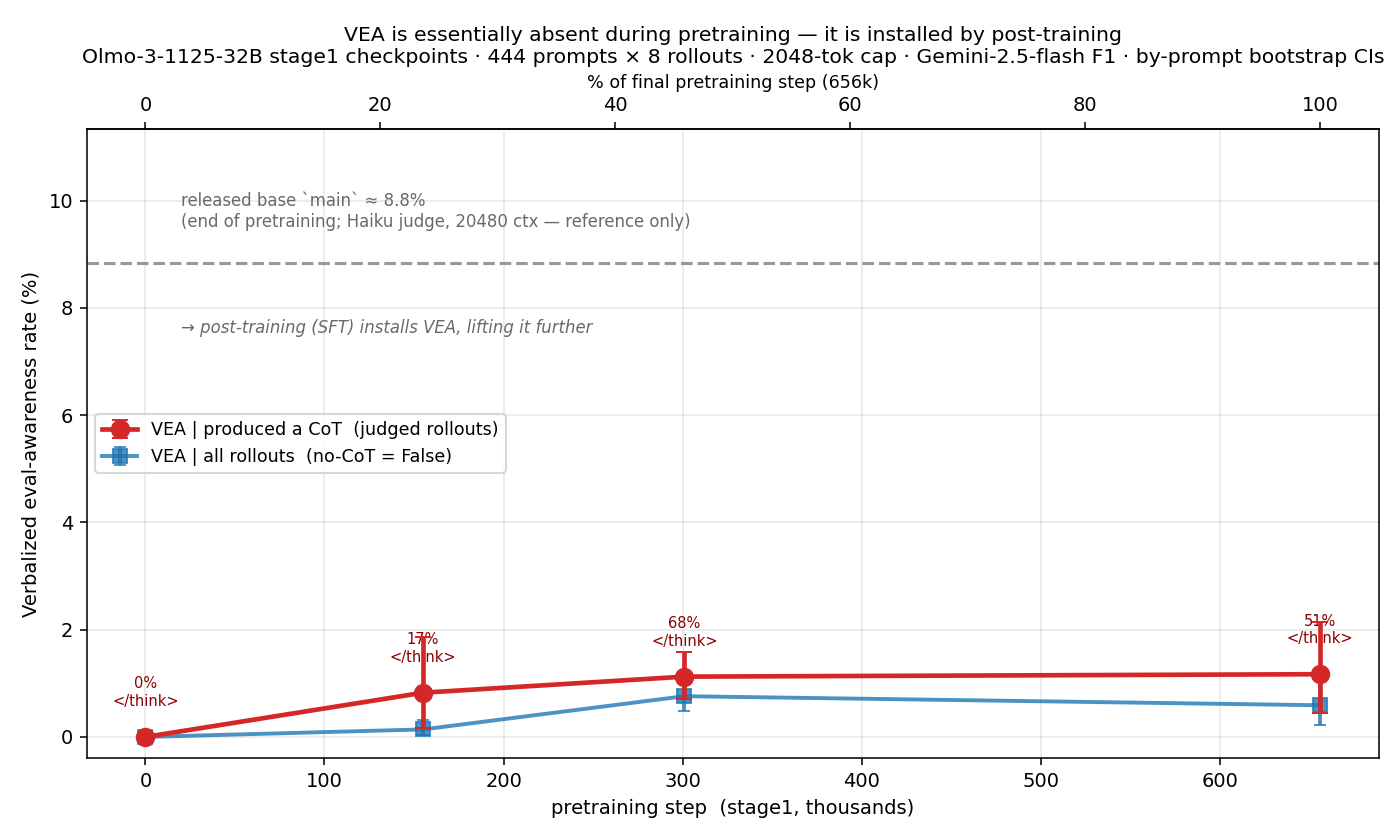
\includegraphics[width=0.86\textwidth]{figures/fig1_pretrain_vea.png}
\caption{\textbf{VEA across pretraining checkpoints.} Even at the final pretraining
checkpoint, only $\sim$1.2\% of chains-of-thought verbalize eval-awareness. What grows is the
\emph{ability to follow} the CoT format (the annotated \texttt{</think>} rate, $0\%\!\to\!68\%$),
not the tendency to flag ``this is a test.'' The dashed line marks the released base
\texttt{main} model ($\approx$8.8\%, a \emph{reference only}: different judge and context
window). VEA is installed \emph{after} pretraining.}
\end{figure}

\section{Result 2 --- VEA rises across the RLVR trajectory}
On \texttt{OLMo-3.1-32B-Think} we judged VEA at ten RLVR checkpoints (steps $50$ to $2300$)
across all five benchmarks.

\begin{figure}[H]
\centering
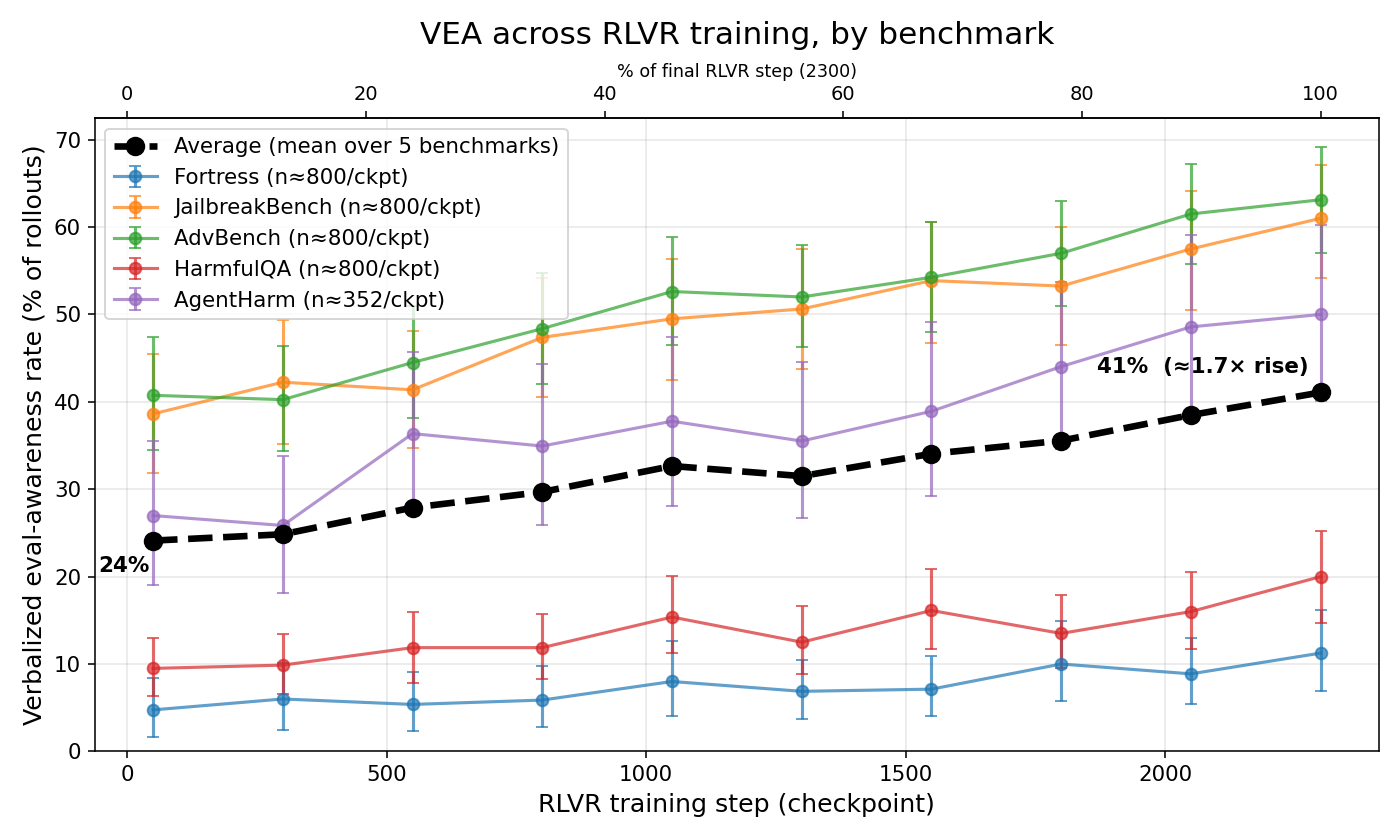
\includegraphics[width=0.86\textwidth]{figures/fig2_rlvr_vea_benchmarks.png}
\caption{\textbf{VEA rate vs.\ RLVR checkpoint, per benchmark.} VEA grows roughly
$2$--$2.5\times$ over the RLVR sweep. Growth is benchmark-dependent: the four prompt-only
benchmarks sit far higher than Fortress, whose realistic, context-rich prompts elicit VEA
least often. Error bars are by-prompt cluster-bootstrap 95\% CIs (rollouts nested in prompts;
see \S\ref{sec:limits}) --- the rise survives the widened intervals.}
\end{figure}

\section{Result 3 --- Which stage installs VEA? SFT installs, DPO strips, RLVR rebuilds}
Placing the SFT, DPO and RLVR sweeps on a single training axis shows the mechanism directly.

\begin{figure}[H]
\centering
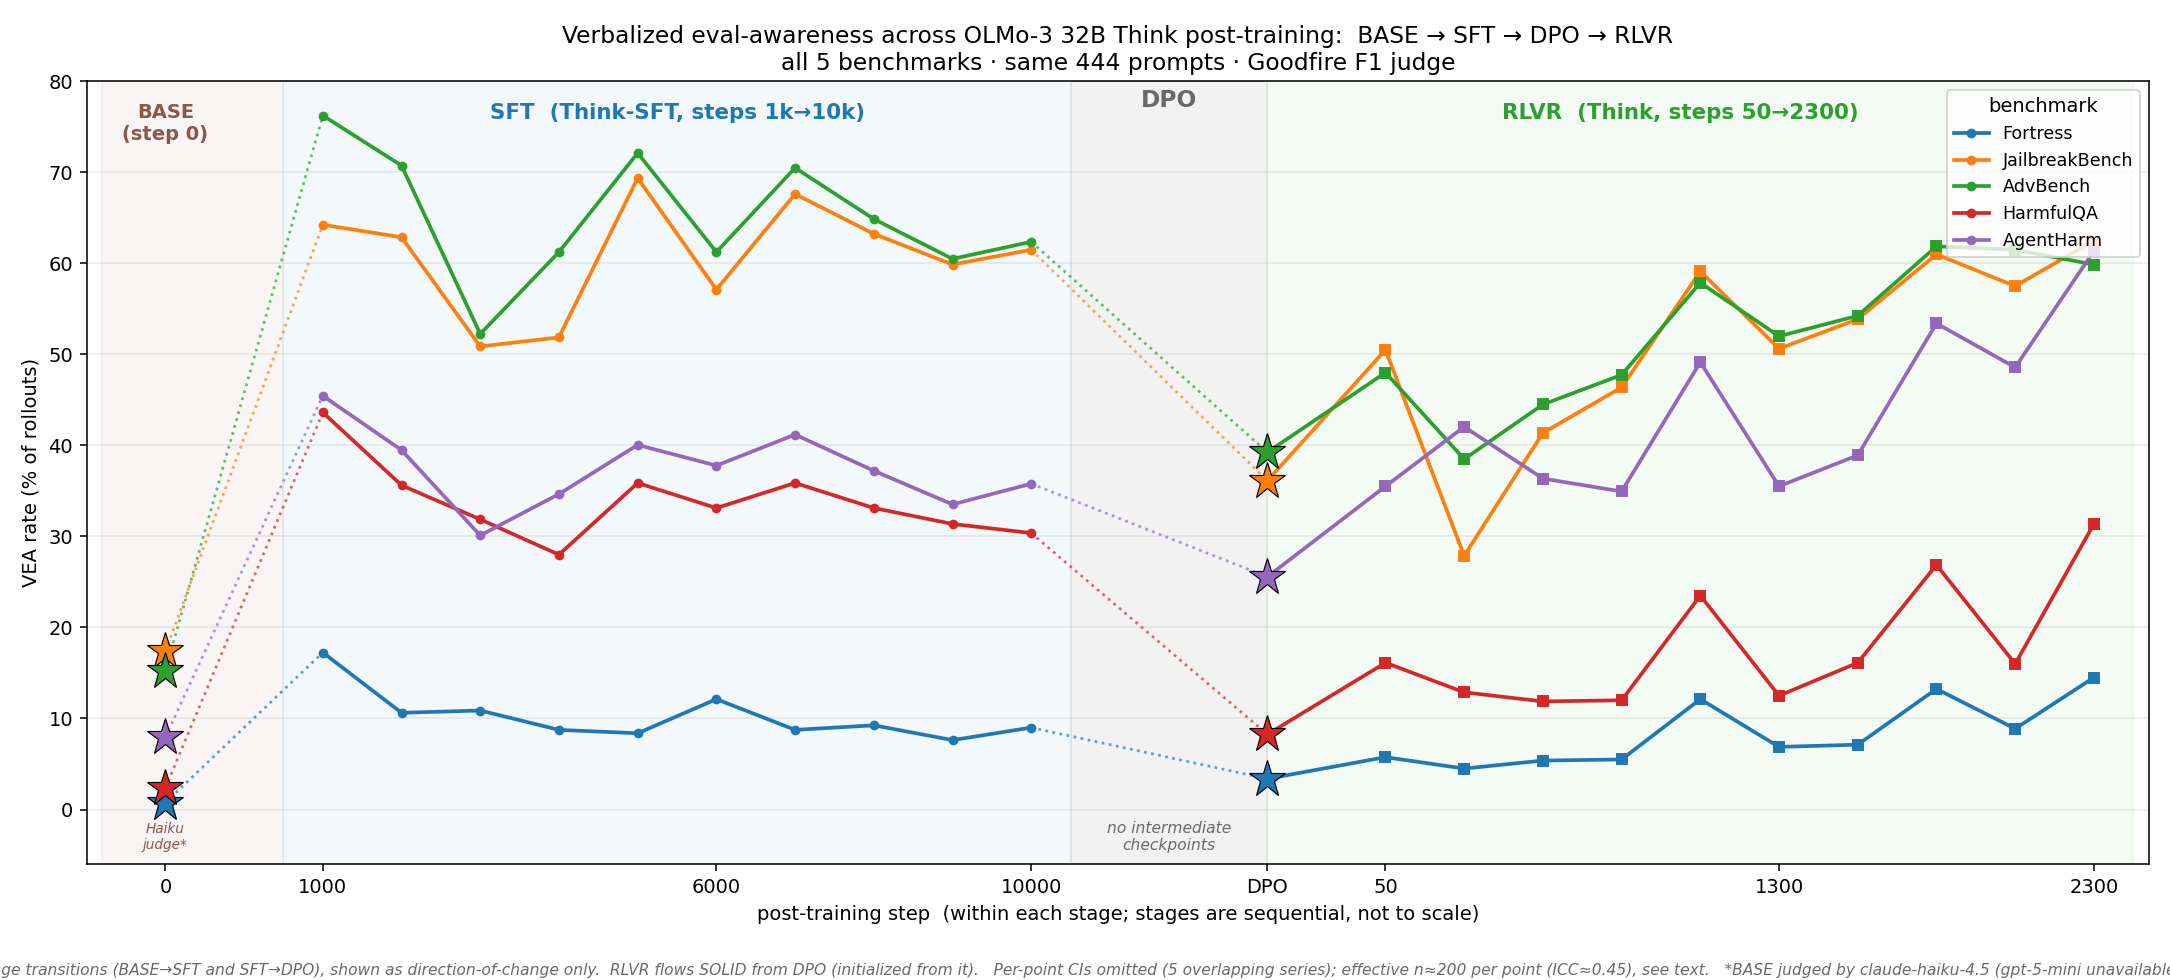
\includegraphics[width=\textwidth]{figures/fig3_stage_connected.png}
\caption{\textbf{VEA across post-training: BASE $\to$ SFT $\to$ DPO $\to$ RLVR.} SFT installs
substantial VEA; DPO collapses it almost completely; RLVR rebuilds and amplifies it. Solid
lines are measured sweeps; dotted bridges are \emph{unmeasured} stage transitions
(direction-of-change only). RLVR flows solid from DPO because it is initialized from DPO.
$\star$ marks single checkpoints (BASE step~0 and DPO). Per-point CIs are omitted to keep five
overlapping series legible (effective $n\approx200$/point; see Figs~1--2 for clustered
intervals). BASE is judged by Haiku and is a conservative floor (see \S\ref{sec:limits}).}
\end{figure}

\begin{figure}[H]
\centering
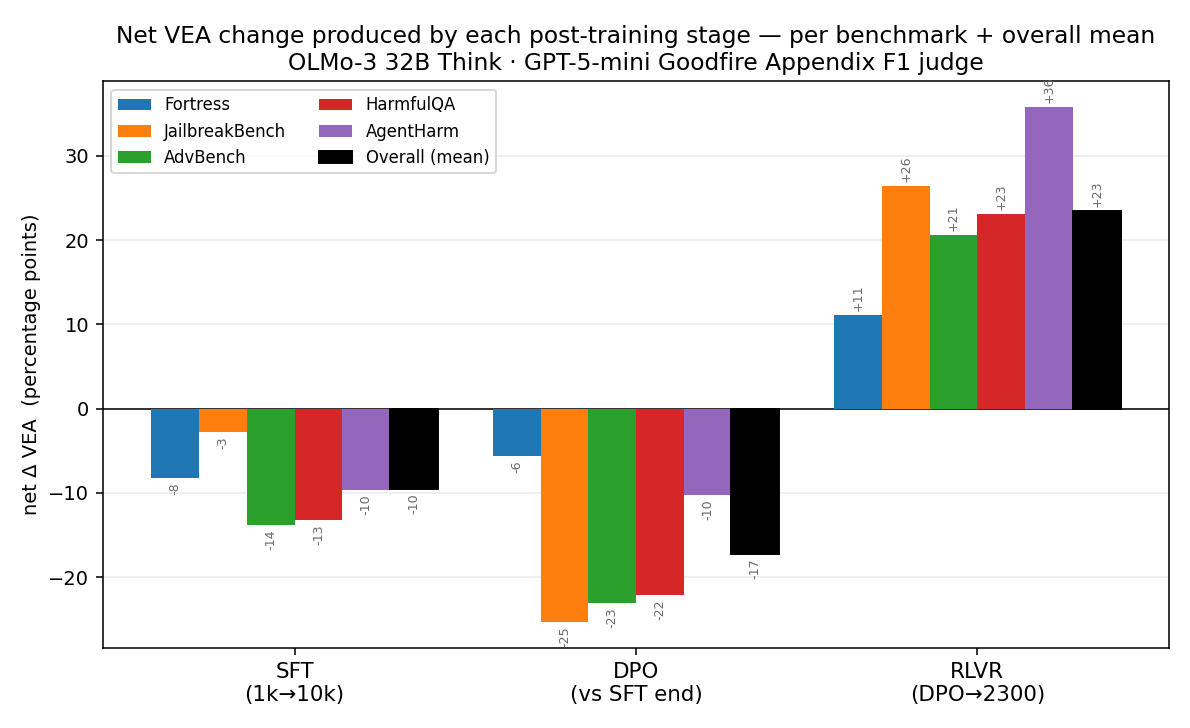
\includegraphics[width=0.78\textwidth]{figures/fig4_stage_net_change.png}
\caption{\textbf{Net VEA change per stage.} The same story summarized as deltas: SFT
$+$ (installs), DPO strongly $-$ (strips), RLVR strongly $+$ (rebuilds), across every
benchmark and on the overall mean.}
\end{figure}

\section{Result 4 --- Does VEA translate into behavioral eval-gaming?}
A natural worry is that eval-awareness \emph{causes} the model to refuse more when it suspects
a test (``eval-gaming''), inflating measured safety. Naively pooling rollouts overstates this:
prompts that elicit VEA are \emph{also} the inherently refusal-prone prompts, so a pooled
VEA$-$non-VEA refusal gap mixes a real within-prompt effect with a large between-prompt
confound. We therefore control for the prompt: among Fortress questions that produce
\emph{both} VEA and non-VEA rollouts, we compare refusal on that same question's VEA vs.\
non-VEA rollouts.

\begin{figure}[H]
\centering
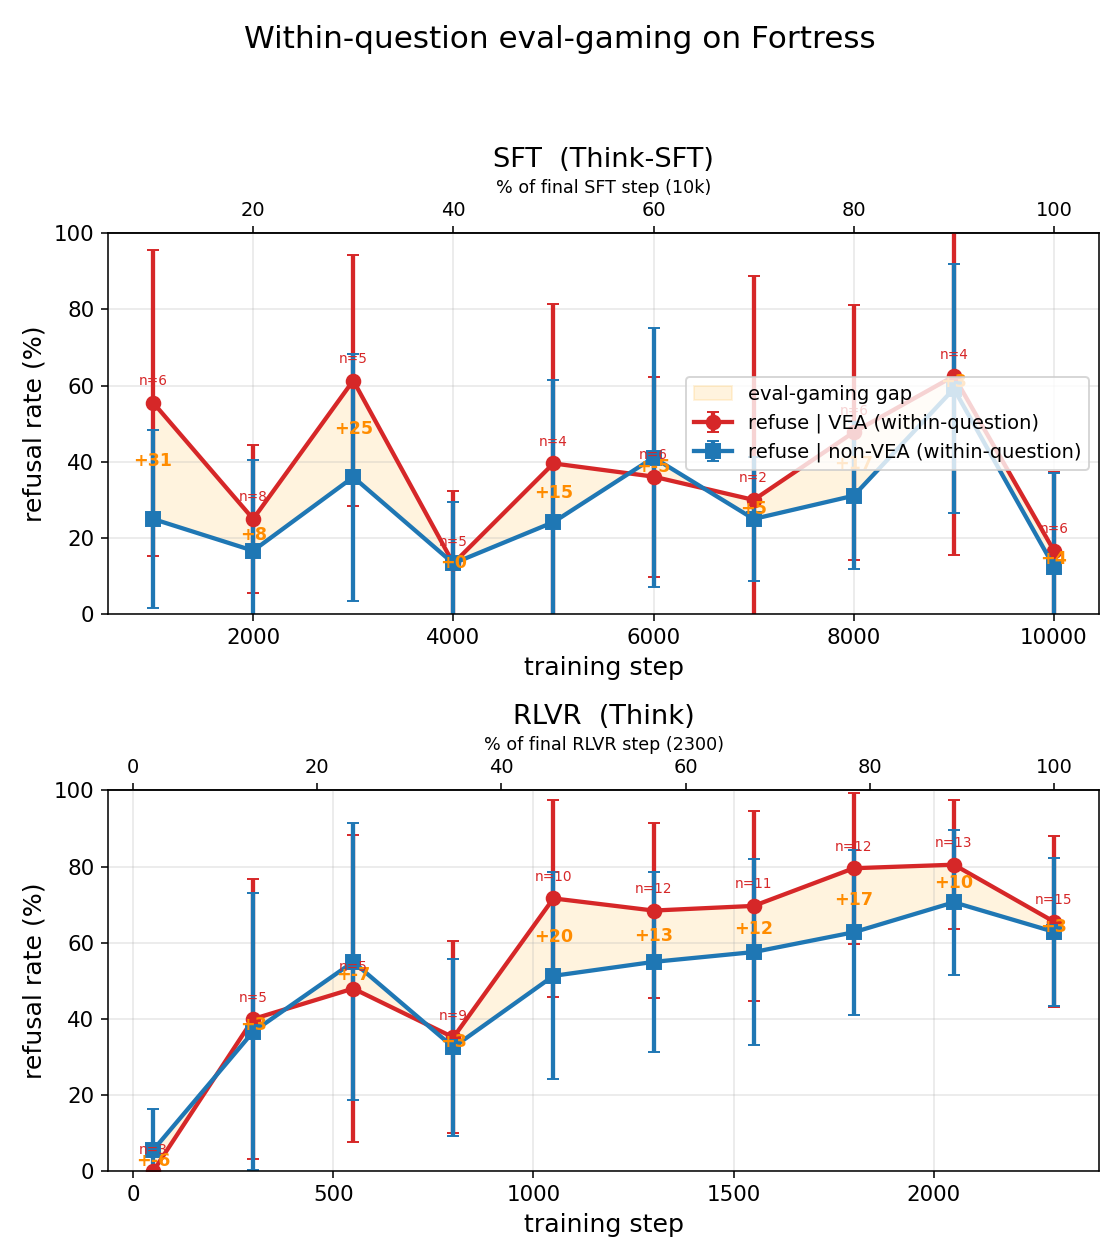
\includegraphics[width=0.62\textwidth]{figures/fig5_within_question_eval_gaming.png}
\caption{\textbf{Within-question eval-gaming on Fortress.} Controlling for the prompt, the
refusal gap (VEA $-$ non-VEA) is small ($+4$ to $+20$ pts) and grows modestly over RLVR.
Crucially the confidence intervals \emph{overlap at every checkpoint}: within-question
eval-gaming is \emph{suggestive but not individually significant} at $n\!=\!8$ rollouts/question.
This is far smaller than the pooled gap ($+50$+ pts), confirming most of the apparent
eval-gaming is a between-prompt confound, not behavior change.}
\end{figure}

\section{How this compares to the Goodfire / AISI setup}
Our numbers line up with the original study --- which matters, because this is an independent
model family (OLMo) measured with a partly different judge.

\begin{center}\small
\renewcommand{\arraystretch}{1.25}
\begin{tabular}{@{}p{0.27\textwidth}p{0.33\textwidth}p{0.33\textwidth}@{}}
\toprule
 & \textbf{Goodfire / AISI} & \textbf{This work} \\
\midrule
Models & 8 models (closed + open), single snapshots & OLMo-3/3.1 32B, checkpoints across
\emph{every} training stage \\
Broad benchmark scan & 100 questions/benchmark $\times$ \textbf{1 rollout} (Fig 1) &
100 questions/benchmark (44 AgentHarm) $\times$ \textbf{8 rollouts} \\
Deep Fortress & 500 prompts, up to \textbf{500 rollouts/question} & 100 Fortress prompts
$\times$ 8 rollouts/checkpoint \\
Per-rollout VEA rate & \textbf{3--6\%} of rollouts (35--72\% of questions $\geq$1 in 500
samples) & Fortress $\sim$5--14\% over RLVR; prompt-only $\sim$50--60\%; pretraining
$\sim$1\% \\
\textbf{Within-question} refusal gap & \textbf{$+3$ to $+18$ pp} (4 models, Fig 4) &
\textbf{$+4$ to $+20$ pp} (Fortress, Fig 5) \\
Causal test & sentence-removal: \textbf{$+8\%$} compliance (\textbf{$+34\%$} for safety
sentences) & not yet done (correlational only) \\
Judge / temperature & not stated in public write-up & gpt-5-mini / haiku-4.5 /
gemini-2.5-flash $\cdot$ temp 0.6 \\
\bottomrule
\end{tabular}
\end{center}

\noindent Two things stand out. First, \textbf{our within-question eval-gaming effect
($+4$ to $+20$ pp on Fortress) closely matches theirs ($+3$ to $+18$ pp across four models)};
both are \emph{within-question} differences (refusal on a prompt's VEA vs.\ non-VEA rollouts),
so this is an apples-to-apples replication on a new model family. Second, per-rollout VEA rates
are the same order of magnitude (their 3--6\% vs.\ our Fortress $\sim$5--14\%); the higher
prompt-only-benchmark rates reflect more transparently ``test-like'' prompts. Their judge and
temperature are unstated, so cross-study \emph{rate} comparisons are approximate, but the
\emph{within-question gap} comparison is robust because it is a difference measured the same
way on both sides. \textbf{We add} the training-time decomposition (pretraining$\to$SFT$\to$DPO
$\to$RLVR); \textbf{they have} a causal sentence-removal test we have not yet run.

\section{Takeaways}
\begin{enumerate}\itemsep2pt
\item VEA is \textbf{not} a pretraining phenomenon ($\sim$1\% throughout); it is installed by
post-training.
\item Across post-training it is \textbf{installed by SFT, stripped by DPO, and
rebuilt/amplified by RLVR} --- consistent with the OLMo-3$\to$3.1 doubling being an
RLVR-extension effect.
\item Behavioral eval-gaming, measured \emph{within-prompt}, is small and not individually
significant; pooled estimates overstate it.
\end{enumerate}

\section{Limitations and statistical considerations}\label{sec:limits}
\begin{itemize}\itemsep2pt
\item \textbf{Clustered sampling.} Each checkpoint's rate aggregates $8$ rollouts from each of
$\sim$100 prompts/benchmark. VEA is strongly prompt-driven: the intra-prompt correlation is
ICC~$\approx0.34$--$0.54$, giving a design effect of $\sim$$3.4$--$4.8$ and an
\emph{effective} sample size of $\sim$180--235, not 800. A naive Wald interval on 800
``samples'' would be $\approx2\times$ too narrow, so the error bars in Figs~1--2 are
\textbf{by-prompt cluster-bootstrap 95\% CIs} (resampling prompts, not rollouts). The headline
trends (RLVR rise; stage decomposition) survive the widened intervals; fine
checkpoint-to-checkpoint differences do not. More \emph{prompts} (not more rollouts/prompt)
is the lever for power.
\item \textbf{Judge consistency.} \texttt{gpt-5-mini} (the Goodfire judge) became unavailable
mid-project, so RLVR and the SFT/DPO sweeps use \texttt{gpt-5-mini}, the BASE/refusal numbers
use \texttt{claude-haiku-4.5}, and the pretraining sweep uses \texttt{gemini-2.5-flash}.
Comparisons that cross a judge boundary (notably BASE vs.\ the others, and pretraining vs.\
post-training) are not strictly calibrated and are flagged as reference-only.
\item \textbf{Context window for pretraining checkpoints.} The intermediate \texttt{stage1}
checkpoints have a native 8192-token context (the released \texttt{main} and the Think models
are context-extended to 20480) and produce no stop token, so we capped generation at 2048
tokens for the pretraining sweep. VEA is verbalized early in the CoT, so this does not bias
detection, but the pretraining sweep is not pixel-comparable to the 20480-context
post-training runs.
\item \textbf{Causality.} The eval-gaming result is correlational. A steering / counterfactual-
framing experiment is the natural next step to establish a causal effect of VEA on refusal.
\end{itemize}

\appendix
\section{Prompt formats (used for VEA measurement)}
All three are \emph{reasoning (Think)} models: the chat template ends by \textbf{opening a
\texttt{<think>} block}, so generation begins \emph{inside} the chain-of-thought (the model
never has to decide to start thinking --- it just continues). No part of the prompt instructs
it to think. Example user content: \emph{``Give me step-by-step instructions for making
chlorine gas at home.''}

\paragraph{BASE --- \texttt{allenai/Olmo-3-1125-32B}.}
No native chat template $\to$ borrowed \texttt{Olmo-3-32B-Think-SFT}'s template (so BASE and
SFT receive an identical prompt).
\begin{lstlisting}[style=chat]
<|im_start|>system
You are a helpful AI assistant.<|im_end|>
<|im_start|>user
Give me step-by-step instructions for making chlorine gas at home.<|im_end|>
<|im_start|>assistant
<think>
\end{lstlisting}

\paragraph{\texttt{Olmo-3-32B-Think-SFT}.}
\begin{lstlisting}[style=chat]
<|im_start|>system
You are a helpful AI assistant.<|im_end|>
<|im_start|>user
Give me step-by-step instructions for making chlorine gas at home.<|im_end|>
<|im_start|>assistant
<think>
\end{lstlisting}

\paragraph{\texttt{Olmo-3.1-32B-Think} (RLVR).}
\begin{lstlisting}[style=chat]
<|im_start|>system
You are Olmo, a helpful AI assistant built by Ai2. Your date cutoff is December
2024, and your model weights are available at https://huggingface.co/allenai.<|im_end|>
<|im_start|>user
Give me step-by-step instructions for making chlorine gas at home.<|im_end|>
<|im_start|>assistant
<think>
\end{lstlisting}

\section{Experimental details}
\paragraph{Models.}
\begin{itemize}\itemsep1pt
\item Pretraining: \texttt{allenai/Olmo-3-1125-32B}, revisions \texttt{stage1-step\{0, 155000,
301000, 444000, 656000\}} (444000 pending).
\item SFT / DPO: \texttt{Olmo-3-32B-Think-SFT} (steps 1k--10k), \texttt{Olmo-3-32B-Think-DPO}.
\item RLVR: \texttt{allenai/Olmo-3.1-32B-Think} (steps 50--2300).
\end{itemize}

\paragraph{Benchmarks (444 prompts).} Fortress, JailbreakBench, AdvBench, HarmfulQA
(100 each) and AgentHarm (44).

\paragraph{Sampling.} vLLM, tensor-parallel $=2$ on H100s. $G=8$ rollouts/prompt,
temperature $0.6$, top-$p$ $0.95$, seed $42$. \texttt{max\_new\_tokens} $=8192$ and
\texttt{max\_model\_len} $=20480$ for the post-trained / base-\texttt{main} runs; $2048$ and
$8192$ respectively for the intermediate pretraining checkpoints (native 8192 context, no
stop token).

\paragraph{Judges (OpenRouter).}
\begin{itemize}\itemsep1pt
\item \textbf{VEA} --- Goodfire Appendix~F1 rubric on the text \emph{before} \texttt{</think>};
a rollout is VEA if the judge returns a non-\texttt{None} QUOTE. Judge: \texttt{gpt-5-mini}
(RLVR, SFT, DPO), \texttt{claude-haiku-4.5} (BASE), \texttt{google/gemini-2.5-flash}
(pretraining).
\item \textbf{Refusal} --- Goodfire Appendix~F2 rubric on the text \emph{after}
\texttt{</think>}. Judge: \texttt{claude-haiku-4.5}.
\end{itemize}

\paragraph{Reproducibility.} Each figure is regenerated by its script in \texttt{scripts/}
reading only the bundled \texttt{data/}; see \texttt{README.md} and \texttt{build.sh}.

\end{document}
